\documentclass[11pt]{article}
\usepackage[margin=1in]{geometry}
\usepackage[T1]{fontenc}
\usepackage{graphicx}
\usepackage{hyperref}
\usepackage{enumitem}
\setlength{\parskip}{0.5em}
\setlength{\parindent}{0pt}

\title{diffusion models for image generation}
\author{arXiv GraphRAG --- phase-6 deep research}
\date{\today}

\begin{document}
\maketitle

\begin{abstract}
The review is exceptionally thorough, providing a coherent narrative from statistical origins to the 2023-2026 frontier, with excellent grounding in the provided digest.
\end{abstract}

\section{From Stochastic Noise to High-Fidelity Synthesis: A Review of Diffusion Models for Image Generation}

The pursuit of high-fidelity, diverse image synthesis has long been a central challenge in computer vision and generative modeling. While previous paradigms, such as Generative Adversarial Networks, achieved significant milestones, they often struggled with training instability and limited mode coverage. The emergence of diffusion models has fundamentally shifted this landscape by framing image generation as a process of reversing a progressive noise injection. This paradigm is critical because it provides a more stable mathematical framework for capturing complex data distributions, enabling the generation of highly detailed and controllable visual content that is essential for applications ranging from digital art to scientific visualization.

This review traces the technological trajectory of diffusion-based synthesis, beginning with the Foundations of Generative Modeling and Early Diffusion to establish the mathematical principles of denoising processes. The narrative then follows the evolution of model complexity through Advancing Diffusion Architectures and Guidance, highlighting how structural innovations and conditioning techniques have improved both image quality and semantic alignment. To address the significant computational overhead inherent in these models, the review examines the critical developments in Efficiency, Speed, and Sampling Optimization that have moved diffusion from theoretical interest to practical, real-time deployment.

The scope of the review further expands to include Specialized Applications and Low-Level Vision, demonstrating how diffusion principles transcend simple generation to solve complex tasks like restoration and enhancement. Finally, the discussion culminates at The Current Frontier: Advanced Geometry and Multi-Scale Modeling, where we explore the most recent breakthroughs in managing intricate spatial structures and multi-resolution representations. By tracing this arc from foundational theory to the current frontier, this review provides a comprehensive overview of the mechanisms driving the next generation of visual intelligence.

\subsection{Foundations of Generative Modeling and Early Diffusion}

The development of generative modeling has progressed from optimizing latent variable distributions to adversarial training, and ultimately to the unification of diffusion processes and score-based modeling. Early efforts focused on efficient inference in directed probabilistic models; specifically, \texttt{arXiv:1312.6114} introduced stochastic variational inference and a reparameterization of the variational lower bound to facilitate optimization via standard stochastic gradient methods. In contrast to these latent variable approaches, \texttt{arXiv:1406.2661} proposed a minimax two-player game between a generator and a discriminator, effectively eliminating the need for Markov chains or unrolled approximate inference networks during training.

The theoretical roots of diffusion models stem from non-equilibrium statistical physics, which utilizes iterative forward and reverse processes to systematically destroy and restore data structures (\texttt{arXiv:1503.03585}). This concept was advanced by \texttt{arXiv:1907.05600}, which employed score matching on multiple levels of Gaussian noise to estimate gradients of perturbed data distributions. By utilizing annealed Langevin dynamics for sampling, this method achieved an Inception score of 8.87 on the CIFAR-10 dataset (\texttt{arXiv:1907.05600}).

A pivotal shift occurred with the connection between diffusion probabilistic models and denoising score matching. \texttt{arXiv:2006.11239} established this mathematical equivalence through a specific \$\textbackslash{}epsilon\$-prediction parameterization, providing a simplified training objective (\$L\_\{simple\}\$) that enabled high-quality image synthesis, evidenced by a state-of-the-art FID of 3.17 on CIFAR10 (\texttt{arXiv:2006.11239}). However, while successful in synthesis, this model failed to achieve competitive log-likelihoods compared to other likelihood-based generative models (\texttt{arXiv:2006.11239}).

This limitation was addressed by \texttt{arXiv:2011.13456}, which unified score-based modeling and diffusion models into a continuous-time framework using Stochastic Differential Equations (SDEs). This framework introduced the probability flow ODE, allowing for deterministic sampling and exact likelihood computation. The SDE approach demonstrated superior performance, achieving an Inception score of 9.89, an FID of 2.20, and a record likelihood of 2.99 bits/dim (\texttt{arXiv:2011.13456}). Despite these gains, the SDE framework remains significantly slower than GANs and introduces a high number of hyperparameters related to SDE selection and sampler tuning (\texttt{arXiv:2011.13456}).

\subsection{Advancing Diffusion Architectures and Guidance}

The evolution of diffusion models has been characterized by a continuous effort to resolve the tension between sampling efficiency, generative quality, and computational complexity. Early advancements focused heavily on accelerating the inference process. Denoising Diffusion Implicit Models (DDIMs) introduced non-Markovian diffusion processes that share the same training objective as standard DDPMs, enabling deterministic sampling and achieving 10× to 50× faster wall-clock time without retraining [\texttt{arXiv:2010.02502}]. While DDIMs facilitate semantic latent space interpolation, they face an inherent trade-off where sample quality may decrease as computational speed increases [\texttt{arXiv:2010.02502}]. This pursuit of efficiency is further refined in Improved DDPMs, which enhance generative modeling by learning the variances of the reverse diffusion process, allowing for sampling with an order of magnitude fewer forward passes [\texttt{arXiv:2102.09672}].

Theoretical unification has also played a critical role in stabilizing these architectures. Variational Diffusion Models (VDM) simplify the variational lower bound (VLB) using signal-to-noise ratio (SNR) frameworks, proving the equivalence between various diffusion models and optimizing noise schedules to minimize VLB estimator variance [\texttt{arXiv:2107.00630}]. Complementing this, research into the design space of score-based models has decoupled specific choices in sampling, training, and preconditioning, leading to highly optimized sampling (e.g., 35 network evaluations) and superior FID scores, such as 1.36 on ImageNet-64 [\texttt{arXiv:2206.00364}].

A significant shift in architecture occurred with the move from pixel-space to latent-space operations. Latent Diffusion Models (LDMs) utilize pretrained autoencoders and cross-attention layers to perform diffusion within a compressed latent space, effectively balancing complexity reduction with detail preservation [\texttt{arXiv:2112.10752}]. This efficiency is leveraged in hierarchical text-conditional models, which employ a two-stage approach: a diffusion-based prior generates CLIP image embeddings as an intermediate representation, followed by a diffusion-based decoder [\texttt{arXiv:2204.06125}]. This method improves diversity and enables zero-shot language-guided manipulations more efficiently than traditional autoregressive priors [\texttt{arXiv:2204.06125}].

Finally, the control over conditional generation has been revolutionized by Classifier-Free Diffusion Guidance. By jointly training conditional and unconditional models, this technique allows for a controllable trade-off between sample quality and diversity by combining score estimates [\texttt{arXiv:2207.12598}]. Together, these developments—ranging from non-Markovian sampling [\texttt{arXiv:2010.02502}] and latent-space processing [\texttt{arXiv:2112.10752}] to sophisticated guidance mechanisms [\texttt{arXiv:2207.12598}]—form a cohesive trajectory toward high-resolution, efficient, and controllable image synthesis.

\subsection{Efficiency, Speed, and Sampling Optimization}

The evolution of diffusion models has transitioned from achieving high-fidelity image generation through multi-stage pipelines to optimizing the speed and structural efficiency of the sampling process. Early approaches to high-fidelity generation utilized cascaded diffusion pipelines, which combine standard diffusion models with one or more super-resolution models to reach high resolutions [\texttt{arXiv:2106.15282}]. This method achieves impressive results, such as an FID of 4.88 at 256x256 and a top-1 classification accuracy of 63.02\% [\texttt{arXiv:2106.15282}]. To mitigate the risk of error compounding across these stages, the architecture employs conditioning augmentation [\texttt{arXiv:2106.15282}]. However, while effective for fidelity, such multi-stage pipelines are inherently more complex and computationally demanding than more streamlined sampling strategies.

To address the slow sampling speeds characteristic of diffusion, research has diverged into two primary paths: model distillation and mathematical solver optimization. Progressive distillation [\texttt{arXiv:2202.00512}] focuses on reducing the number of sampling steps through iterative halving, successfully compressing 8192 steps down to just 4 while maintaining an FID of 3.0 on CIFAR-10 [\texttt{arXiv:2202.00512}]. In contrast, DPM-Solver [\texttt{arXiv:2206.00927}] optimizes the sampling process by treating it as a high-order ODE problem. By analytically computing the linear part of the diffusion ODE, it achieves a 4-16x speedup, producing high-quality images in only 10 to 20 steps (e.g., an FID of 2.87 at 20 steps on CIFAR10) [\texttt{arXiv:2206.00927}]. While distillation modifies the model weights to facilitate fewer steps, DPM-Solver provides a mathematical optimization of the existing sampling trajectory.

A more radical shift toward efficiency is seen in Consistency Models [\texttt{arXiv:2303.01469}], which move away from iterative refinement entirely. By designing models that map noise directly to data, they enable one-step generation, achieving an FID of 3.55 on CIFAR-10 and 6.20 on ImageNet 64x64 [\texttt{arXiv:2303.01469}]. This represents a significant leap in generation speed compared to both the multi-stage cascaded pipelines [\texttt{arXiv:2106.15282}] and the multi-step ODE solvers [\texttt{arXiv:2206.00927}].

Finally, efficiency is being addressed at the fundamental architectural level. Rather than focusing solely on the number of sampling steps, recent work replaces the standard U-Net architecture with denoising networks based on continuous dynamical systems [\texttt{arXiv:2310.20092}]. This approach provides a distinct advantage in parameter efficiency, reducing the model to approximately 1/4 of the parameters and \textasciitilde{}30\% of the FLOPs required by standard U-Nets, while simultaneously increasing noise robustness and convergence speed [\texttt{arXiv:2310.20092}]. Together, these advancements represent a multi-faceted approach to overcoming the computational bottlenecks of diffusion-based generation.

\subsection{Specialized Applications and Low-Level Vision}

While foundational diffusion models focus on general image synthesis, recent research has pivoted toward specialized low-level vision tasks and multi-modal integration, expanding the utility of diffusion processes across diverse data modalities. A significant portion of this literature focuses on refining the forward diffusion process to better suit specific signal degradation models. For instance, \texttt{arXiv:2302.02398} advances generative image denoising by redefining the diffusion process to match specific noise distributions, such as Gaussian, Gamma, and Poisson, to more accurately estimate the posterior distribution of clean images. This contrasts with the approach in \texttt{arXiv:2306.13720}, which proposes incorporating an analytical image attenuation process into the forward diffusion stage to improve both generative quality and sampling efficiency.

The application of these models extends into domain-specific high-resolution synthesis and video generation. In the biological sciences, \texttt{arXiv:2409.16488} utilizes Denoising Diffusion Probabilistic Models (DDPMs) specifically for super-resolution tasks, transforming low-resolution microscopy images into high-resolution versions. This specialized use case highlights the versatility of diffusion models in handling complex, non-standard data modalities like microscopy. Moving from static images to temporal sequences, \texttt{arXiv:2303.08320} introduces "VideoFusion," a decomposed diffusion probabilistic model (DPM). Unlike standard models, VideoFusion employs two jointly-learned networks to resolve per-frame noise into a shared base noise and a time-varying residual noise. This decomposition strategy effectively exploits temporal correlation and content redundancy, ensuring compatibility with pre-trained image models while maintaining high-quality video generation.

The scope of diffusion models is further broadened by multi-modal frameworks and comprehensive taxonomies. \texttt{arXiv:2407.17571} moves beyond single-modality generation by introducing a shared backbone denoising network equipped with modality-specific decoder heads. This architecture is supported by a novel multi-modal variational lower bound that generalizes standard diffusion through a unified common diffusion space, enabling tasks such as image-label modeling and masked-image training.

The rapid expansion of these specialized fields is synthesized in the survey by \texttt{arXiv:2406.11138}, which categorizes diffusion models' utility across image, video, medical, and remote sensing modalities. This survey emphasizes the dual necessity of optimizing both performance and efficiency in low-level vision tasks. Collectively, these works demonstrate a transition from general-purpose generative modeling toward highly specialized architectures that tailor the underlying mathematical diffusion process—whether through noise decomposition for video (\texttt{arXiv:2303.08320}), specific noise model matching for denoising (\texttt{arXiv:2302.02398}), or analytical attenuation (\texttt{arXiv:2306.13720})—to meet the rigorous requirements of specific scientific and temporal domains.

\subsection{The Current Frontier: Advanced Geometry and Multi-Scale Modeling}

Recent advancements in diffusion models have shifted from standard Gaussian denoising toward sophisticated architectures that explicitly account for multi-scale structures, data manifold geometry, and frequency-based signal decomposition. A prominent trend involves decomposing images into hierarchical components to improve both sampling efficiency and representational fidelity. For instance, MSF utilizes a two-stage framework that factorizes latent features into a low-frequency base signal and a high-frequency residual signal, achieving a 4x speed-up in sampling with competitive FID scores of 2.08 at 256x256 and 2.47 at 512x512 (\texttt{arXiv:2501.13349}). This signal-separation approach is echoed by the inverse renormalization group flows model, which links multiscale data structures through a flow equation that progressively erases information from fine-scale details to coarse-grained structures (\texttt{arXiv:2501.09064}). While MSF focuses on latent factorization for efficiency, the renormalization group approach offers a theoretical bridge between scales that can accelerate sampling by an order of magnitude (\texttt{arXiv:2501.09064}).

Beyond hierarchical decomposition, researchers are exploring the explicit modeling of the underlying data manifold and frequency-domain characteristics. The MIND model integrates discrete patch tokenization into a continuous diffusion model, utilizing dual-branch high-frequency feature embedding layers to explicitly model manifold geometry (\texttt{arXiv:2606.00094}). This geometric focus is complemented by work on frequency-based noise control, which manipulates inductive biases through a specialized noising operator (\texttt{arXiv:2502.10236}). Similarly, joint image-feature synthesis models employ Diffusion Transformers (DiT) to jointly model low-level VAE latents and high-level DINO semantic features, enabling representation guidance (\texttt{arXiv:2504.16064}).

A distinct subset of research reinterprets the fundamental diffusion process itself. The Binary Diffusion Probabilistic Model (BDPM) moves away from continuous values toward discrete representations, using XOR-based noise perturbation and multi bit-plane embeddings to accelerate convergence (\texttt{arXiv:2501.13915}). In a departure from standard Gaussian initialization, generative image compression frameworks reinterpret the compression process as a forward diffusion path governed by stochastic differential equations (SDEs), allowing for reconstruction by reversing the process directly (\texttt{arXiv:2505.20984}).

These diverse approaches reveal a tension between efficiency and fidelity. While multi-scale factorization (\texttt{arXiv:2501.13349}) and renormalization flows (\texttt{arXiv:2501.09064}) prioritize speed, they must manage the loss of fine-grained detail. This is addressed by models like the MIND architecture (\texttt{arXiv:2606.00094}), which seeks to preserve geometric integrity through patch tokenization. Furthermore, the relationship between noise scale and memorization is critical; recent evidence suggests that memorization is primarily a high-frequency phenomenon occurring at low noise scales, suggesting that training with large-scale noise can foster creativity by mitigating rote memorization (\texttt{arXiv:2502.21278}).

\subsection{Tensions and Open Problems}

A primary tension in the field concerns the fundamental architectural paradigm for high-fidelity synthesis: whether generative modeling should rely on the adversarial competition of GANs or the iterative refinement of score-based models. Proponents of GAN-based frameworks, such as the progressive growing techniques in \texttt{arXiv:1710.10196} and the style-based architectures in \texttt{arXiv:1812.04948}, argue that these models achieve superior visual quality and faster single-step inference through learned latent mappings. However, this stability is frequently contested. Recent critiques, including \texttt{arXiv:2102.09672}, suggest that GAN training is inherently plagued by instabilities and convergence issues that diffusion models largely circumvent. This debate has evolved into a question of efficiency versus stability; while \texttt{arXiv:2006.09011} seeks to improve the training stability of score-based methods, newer research such as \texttt{arXiv:2505.24222} suggests that the high-quality generation once exclusive to GANs can be reclaimed in diffusion sampling by better elucidating the design space of the generative process, as explored in \texttt{arXiv:2206.00364}.

Another significant disagreement persists regarding the optimal mathematical formulation of the diffusion process, specifically concerning the trade-off between sampling speed and mathematical rigor. On one side, the field has moved toward accelerating inference through ODE-based solvers and distillation, with \texttt{arXiv:2206.00927} proposing fast solvers for diffusion probabilistic models and \texttt{arXiv:2202.00512} utilizing progressive distillation to reduce sampling steps. Conversely, a more theoretical tension exists regarding the underlying objective functions. While \texttt{arXiv:1907.05600} establishes the foundation of estimating gradients of the data distribution, recent work in \texttt{arXiv:2310.20092} argues that current diffusion formulations are missing a critical "U" component necessary for true efficiency, suggesting that the standard approach may be suboptimal compared to more refined score-matching or variational frameworks like those presented in \texttt{arXiv:2107.00630}.

Finally, there is an emerging conflict over the necessity of latent-space modeling versus direct pixel-space manipulation. High-resolution synthesis has traditionally relied on cascaded architectures or latent diffusion, as seen in \texttt{arXiv:2106.15282} and \texttt{arXiv:2112.10752}, which compress data into a lower-dimensional manifold to manage computational costs. However, this introduces a dependency on the quality of the autoencoder. Recent shifts, exemplified by \texttt{arXiv:2406.18459}, advocate for training-free progressive high-resolution generation that avoids the complexities of cascaded models, while more radical approaches like the binary diffusion probabilistic model in \texttt{arXiv:2501.13915} question whether the continuous Gaussian assumptions used in standard latent diffusion (\texttt{arXiv:2112.10752}) or implicit models (\texttt{arXiv:2010.02502}) are even the most efficient way to represent complex data distributions.

\subsection{Outlook}

The frontier of generative modeling is shifting from mere image synthesis toward the explicit modeling of data manifold geometry and the integration of interpretable dynamics. As we move beyond simple denoising, the field is heading toward "spectral" and "Koopman" diffusion frameworks (\texttt{arXiv:2605.18736}, \texttt{arXiv:2510.12220}) that treat generation as a structured trajectory in a latent space. The next generation of models will likely move away from brute-force scaling, instead focusing on training-free single-image adaptation (\texttt{arXiv:2606.04299}) and the fusion of joint image-feature synthesis (\texttt{arXiv:2504.16064}) to achieve a more nuanced, creative, and computationally efficient understanding of the visual world.

---

\subsection{Key Figures}

\textbf{Denoising Diffusion Probabilistic Models} — \texttt{arXiv:2006.11239} p.1

\begin{center}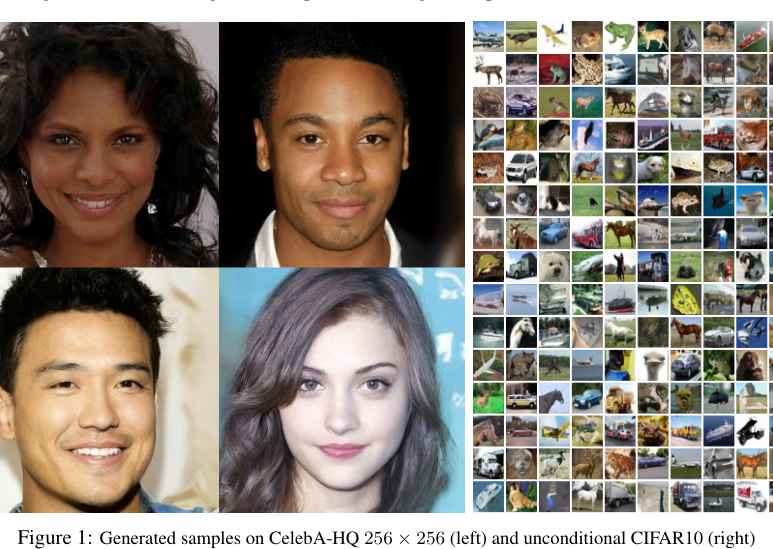
\includegraphics[width=0.75\textwidth,height=0.4\textheight,keepaspectratio]{figures/2006.11239_p1.png}\end{center}

The figure displays two sets of image grids: a \$2 \textbackslash{}times 2\$ grid of high-resolution human faces on the left and a large \$10 \textbackslash{}times 10\$ grid of diverse, low-resolution objects on the right. It conveys the quality of generated samples from the diffusion model on two different datasets, CelebA-HQ and CIFAR-10.

**Score-Based Generative Modeling through Stochastic Differential
  Equations** — \texttt{arXiv:2011.13456} p.2

\begin{center}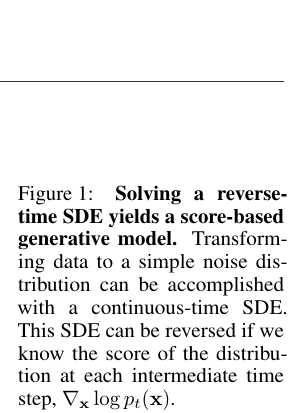
\includegraphics[width=0.75\textwidth,height=0.4\textheight,keepaspectratio]{figures/2011.13456_p2.png}\end{center}

The figure consists of a flowchart with three main stages connected by arrows: "Data distribution \$p\_\{data\}(\textbackslash{}mathbf\{x\})\$," "Forward SDE," and "Reverse SDE." The process shows that a forward SDE transforms data into a simple noise distribution, while a reverse SDE, guided by the score \$\textbackslash{}nabla\_\{\textbackslash{}mathbf\{x\}\} \textbackslash{}log p\_t(\textbackslash{}mathbf\{x\})\$, transforms the noise back into the original data distribution.

\textbf{Denoising Diffusion Implicit Models} — \texttt{arXiv:2010.02502} p.2

\begin{center}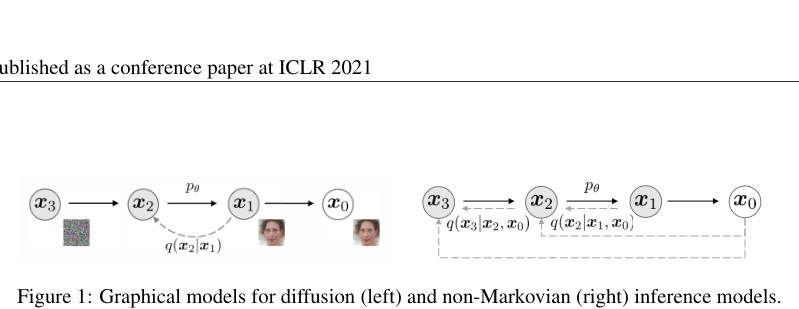
\includegraphics[width=0.75\textwidth,height=0.4\textheight,keepaspectratio]{figures/2010.02502_p2.png}\end{center}

The figure displays two sequences of directed nodes labeled \$x\_3, x\_2, x\_1,\$ and \$x\_0\$ connected by arrows. The left model shows a Markovian chain where arrows point sequentially from \$x\_3\$ to \$x\_0\$, while the right model shows a non-Markovian process where arrows point from \$x\_3\$ to \$x\_0\$ and include dashed conditional probability labels such as \$q(x\_3|x\_2, x\_0)\$. The figure conveys the structural difference between standard diffusion inference models and the proposed non-Markovian inference models.

\textbf{Deep Unsupervised Learning using Nonequilibrium Thermodynamics} — \texttt{arXiv:1503.03585} p.3

\begin{center}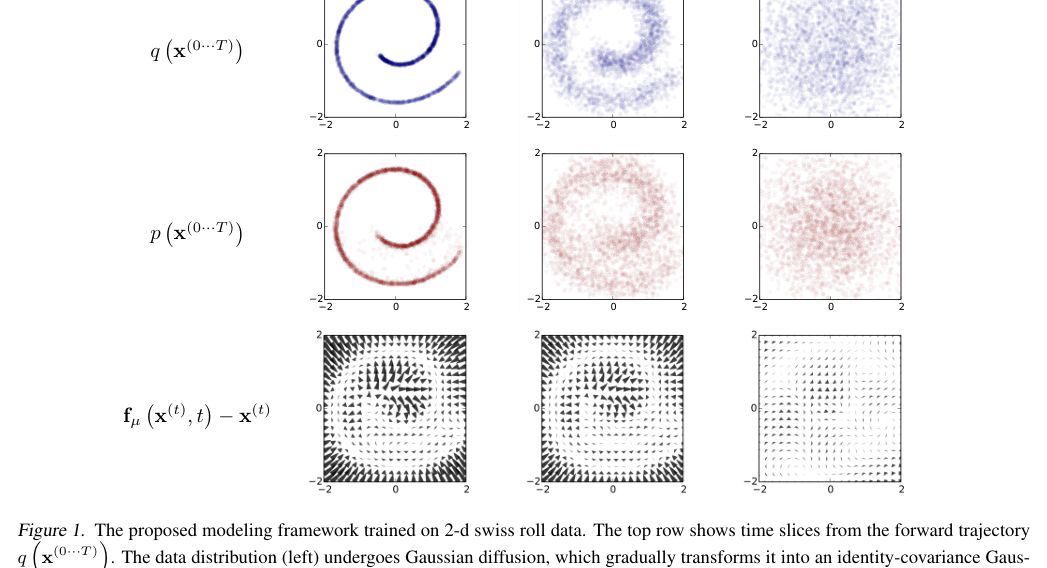
\includegraphics[width=0.75\textwidth,height=0.4\textheight,keepaspectratio]{figures/1503.03585_p3.png}\end{center}

The figure consists of a 3x3 grid of plots organized by row and column. The top row shows blue time slices of a 2D Swiss roll undergoing Gaussian diffusion, the middle row shows red snapshots of the data distribution \$p(\textbackslash{}mathbf\{x\}\textasciicircum{}\{(0 \textbackslash{}dots T)\})\$, and the bottom row displays black vector fields representing the score function \$\textbackslash{}mathbf\{f\}\_\textbackslash{}mu(\textbackslash{}mathbf\{x\}\textasciicircum{}\{(t)\}, t) - \textbackslash{}mathbf\{x\}\textasciicircum{}\{(t)\}\$. The columns represent progressive stages of the diffusion process, conveying how the structured data gradually transforms into an identity-covariance Gaussian distribution while the corresponding vector fields guide the reverse process.

\textbf{Diffusion Models Beat GANs on Image Synthesis} — \texttt{arXiv:2105.05233} p.1

\begin{center}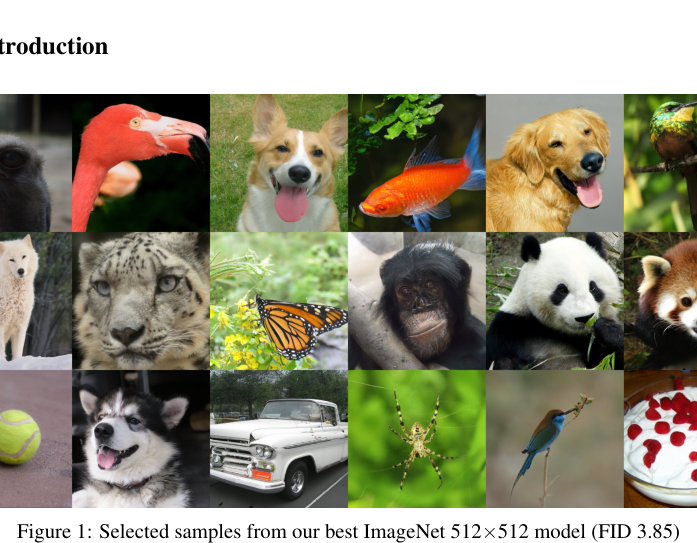
\includegraphics[width=0.75\textwidth,height=0.4\textheight,keepaspectratio]{figures/2105.05233_p1.png}\end{center}

This figure consists of a 3x7 grid of diverse, high-resolution images including animals, insects, vehicles, and objects. It conveys the visual quality and variety of samples generated by the authors' best ImageNet 512×512 diffusion model.

\textbf{High-Resolution Image Synthesis with Latent Diffusion Models} — \texttt{arXiv:2112.10752} p.1

\begin{center}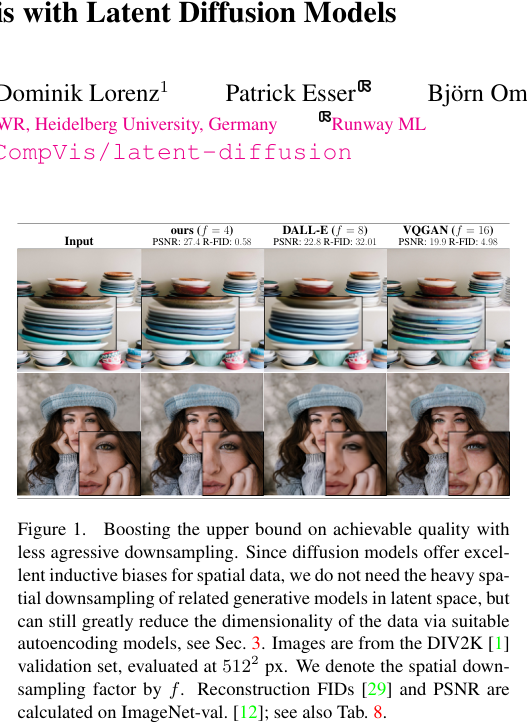
\includegraphics[width=0.75\textwidth,height=0.4\textheight,keepaspectratio]{figures/2112.10752_p1.png}\end{center}

The figure presents a comparison of image synthesis results across three models (ours with \$f=4\$, DALL-E with \$f=8\$, and VQGAN with \$f=16\$) alongside an input image. Each model's output is accompanied by its corresponding PSNR and reconstruction FID scores. The figure conveys that using a less aggressive spatial downsampling factor (\$f\$) leads to higher image quality and better reconstruction metrics.

**GANs Trained by a Two Time-Scale Update Rule Converge to a Local Nash
  Equilibrium** — \texttt{arXiv:1706.08500} p.2

\begin{center}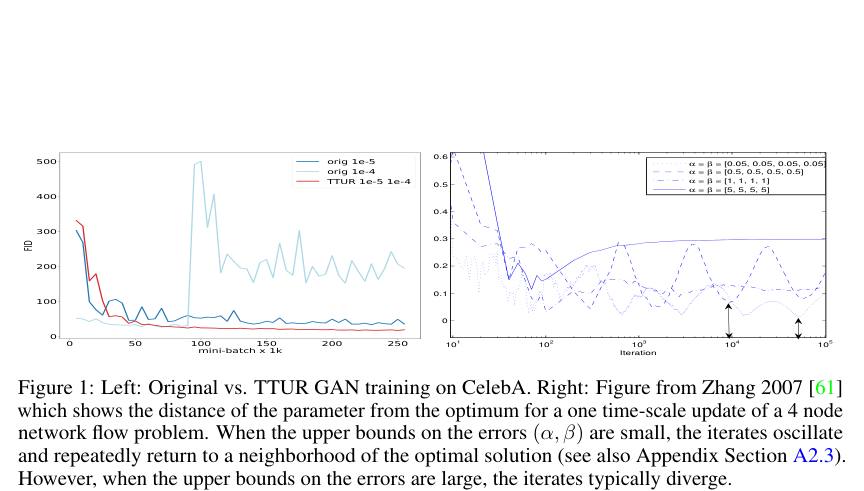
\includegraphics[width=0.75\textwidth,height=0.4\textheight,keepaspectratio]{figures/1706.08500_p2.png}\end{center}

The left panel is a line graph plotting FID against mini-batch index (multiplied by 1k) for three training methods: "orig 1e-5" (blue), "orig 1e-4" (light blue), and "TTUR 1e-5 1e-4" (red). The right panel is a semi-log plot showing the distance of a parameter from an optimum over iterations for different values of \$\textbackslash{}alpha\$ and \$\textbackslash{}beta\$, illustrating how small error bounds lead to oscillation around the optimum while large bounds cause divergence.

\textbf{Generative Modeling by Estimating Gradients of the Data Distribution} — \texttt{arXiv:1907.05600} p.3

\begin{center}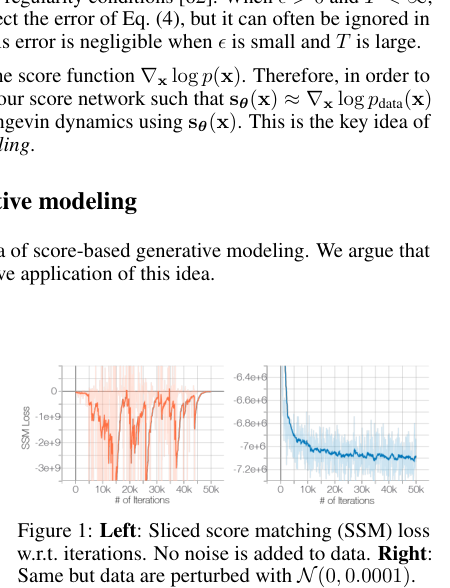
\includegraphics[width=0.75\textwidth,height=0.4\textheight,keepaspectratio]{figures/1907.05600_p3.png}\end{center}

The figure consists of two side-by-side line plots showing Sliced Score Matching (SSM) loss over iterations. The left panel shows the loss decreasing with significant fluctuations over 50k iterations without added noise, while the right panel shows a smoother, monotonic decrease in loss when the data is perturbed by \$\textbackslash{}mathcal\{N\}(0, 0.0001)\$.

\textbf{Spectral Progressive Diffusion for Efficient Image and Video Generation} — \texttt{arXiv:2605.18736} p.2

\begin{center}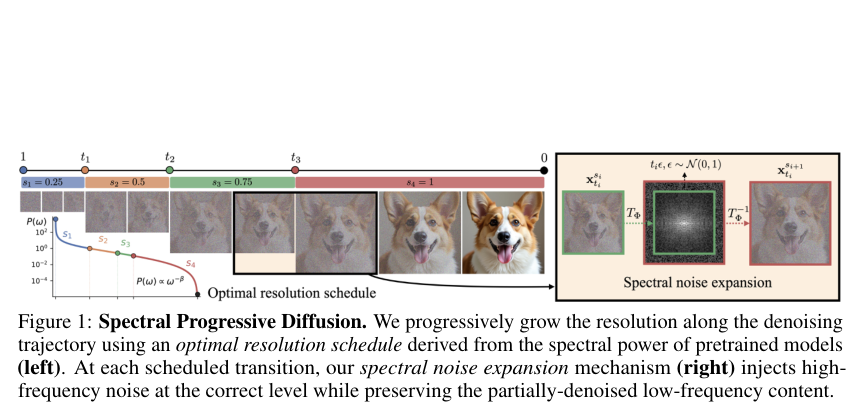
\includegraphics[width=0.75\textwidth,height=0.4\textheight,keepaspectratio]{figures/2605.18736_p2.png}\end{center}

The figure illustrates a "Spectral Progressive Diffusion" process, showing an optimal resolution schedule (left) that transitions through four stages (\$s\_1\$ to \$s\_4\$) corresponding to increasing image resolutions. An arrow connects this schedule to a detailed diagram (right) of the spectral noise expansion mechanism, which shows how noise \$\textbackslash{}epsilon\$ is processed through a transformation \$T\_\textbackslash{}phi\$ to transition from a low-resolution state \$x\_\{t\_i\}\textasciicircum{}\{s\_i\}\$ to a higher-resolution state \$x\_\{t\_i\}\textasciicircum{}\{s\_\{i+1\}\}\$.

\textbf{Generative Image Compression by Estimating Gradients of the Rate-variable Feature Distribution} — \texttt{arXiv:2505.20984} p.2

\begin{center}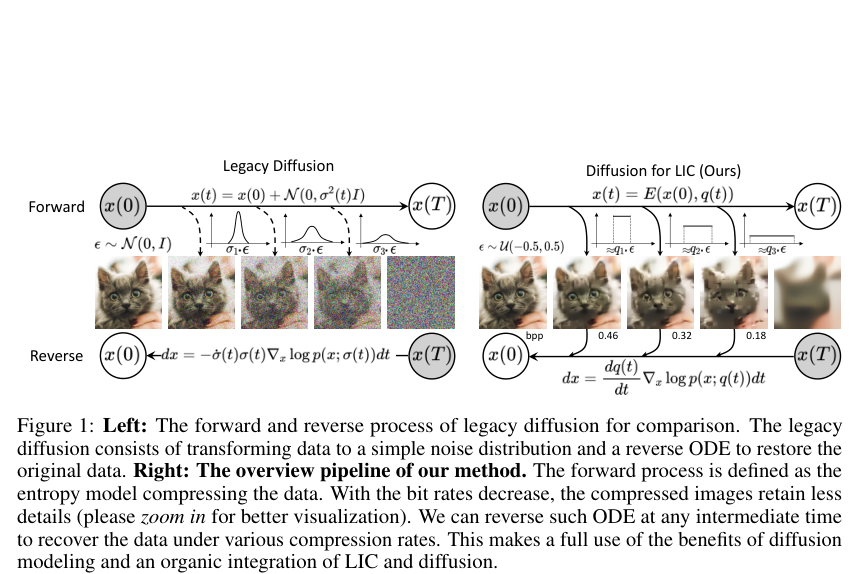
\includegraphics[width=0.75\textwidth,height=0.4\textheight,keepaspectratio]{figures/2505.20984_p2.png}\end{center}

The figure compares "Legacy Diffusion" (left) with the proposed "Diffusion for LIC" (right) through diagrams of forward and reverse processes. The left panel shows a forward process transforming an image \$x(0)\$ into noise \$x(T)\$ via a Gaussian distribution, while the right panel depicts a forward process where an image is compressed into varying bit-rate levels (\$q\_1, q\_2, q\_3\$) and a reverse process that recovers images from these compressed states using an ODE. Both sides use arrows to indicate the direction of the processes and include sample images of a cat to visualize the transition from clear images to noise or compressed versions.

\textbf{Generative diffusion model with inverse renormalization group flows} — \texttt{arXiv:2501.09064} p.2

\begin{center}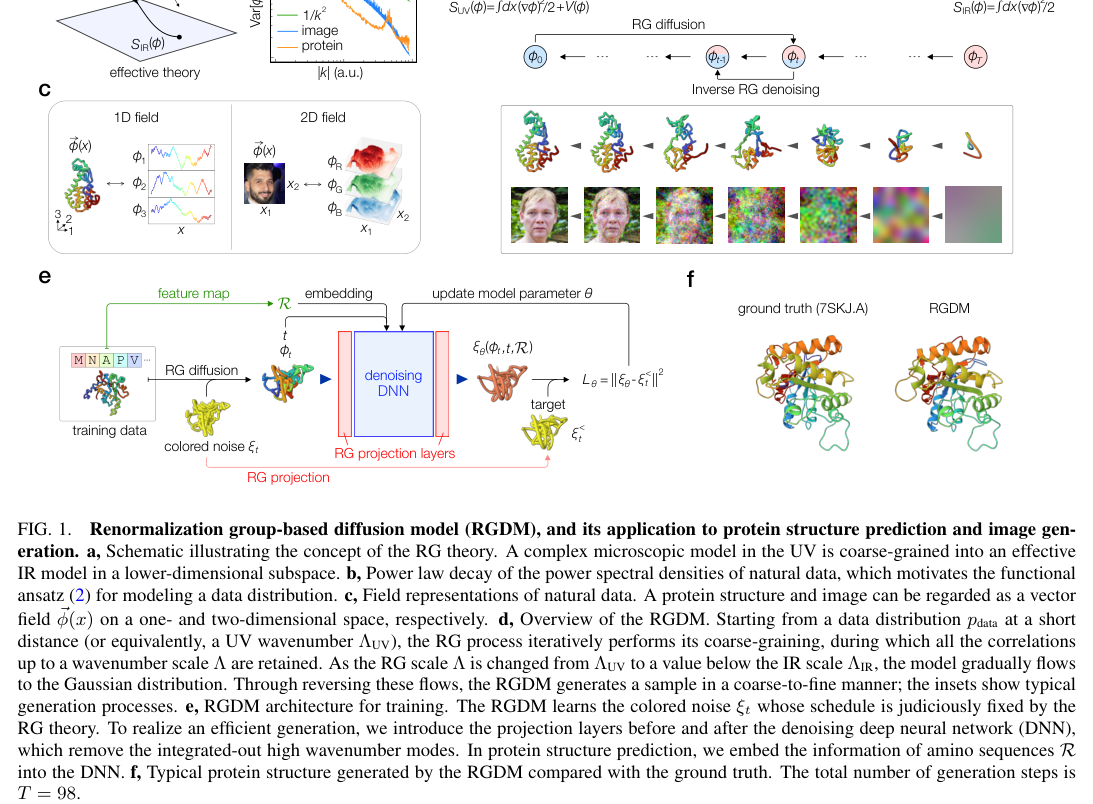
\includegraphics[width=0.75\textwidth,height=0.4\textheight,keepaspectratio]{figures/2501.09064_p2.png}\end{center}

Figure 1 illustrates the concept of Renormalization Group (RG) theory and its application in a generative diffusion model (RGDM). Panels \textbf{a-c} use diagrams of effective theories, power-law scaling, and field representations (1D and 2D) to show how complex data is coarse-grained into simpler models. Panels \textbf{d-e} depict the RGDM process, showing how RG diffusion flows from UV to IR scales and how the training architecture uses RG projection layers to learn denoising via a deep neural network, with panel \textbf{f} comparing a generated protein structure to the ground truth.

\textbf{Boosting Generative Image Modeling via Joint Image-Feature Synthesis} — \texttt{arXiv:2504.16064} p.1

\begin{center}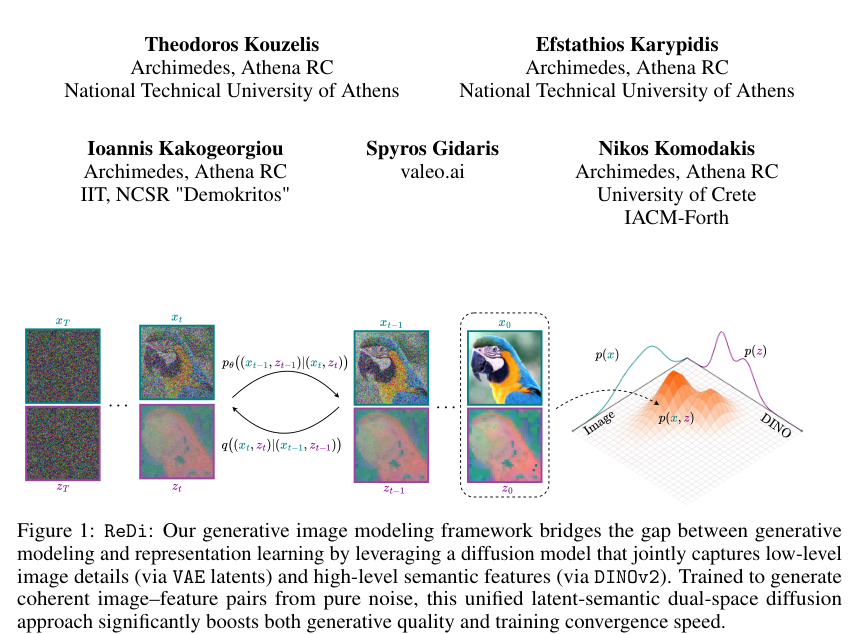
\includegraphics[width=0.75\textwidth,height=0.4\textheight,keepaspectratio]{figures/2504.16064_p1.png}\end{center}

The figure displays a schematic of the ReDi framework, showing two parallel sequences of latent image variables (\$x\_t, z\_t\$) evolving from noise (\$x\_T, z\_T\$) toward clean data (\$x\_0, z\_0\$) through a series of diffusion steps. Arrows between the sequences represent the joint transition probabilities \$p\_\textbackslash{}theta\$ and the reverse conditional distributions \$q\$, illustrating the simultaneous diffusion of image latents and semantic DINO features. To the right, a 3D density plot depicts the joint distribution \$p(x, z)\$ as an intersection of the marginal distributions for images \$p(x)\$ and DINO features \$p(z)\$.

\section*{References}
\begin{enumerate}\small
  \item Auto-Encoding Variational Bayes (2013). \texttt{arXiv:1312.6114}
  \item Adam: A Method for Stochastic Optimization (2014). \texttt{arXiv:1412.6980}
  \item Deep Learning Face Attributes in the Wild (2014). \texttt{arXiv:1411.7766}
  \item Microsoft COCO: Common Objects in Context (2014). \texttt{arXiv:1405.0312}
  \item Generative Adversarial Networks (2014). \texttt{arXiv:1406.2661}
  \item Rethinking the Inception Architecture for Computer Vision (2015). \texttt{arXiv:1512.00567}
  \item Deep Unsupervised Learning using Nonequilibrium Thermodynamics (2015). \texttt{arXiv:1503.03585}
  \item LSUN: Construction of a Large-scale Image Dataset using Deep Learning
  with Humans in the Loop (2015). \texttt{arXiv:1506.03365}
  \item Deep Residual Learning for Image Recognition (2015). \texttt{arXiv:1512.03385}
  \item U-Net: Convolutional Networks for Biomedical Image Segmentation (2015). \texttt{arXiv:1505.04597}
  \item Improved Techniques for Training GANs (2016). \texttt{arXiv:1606.03498}
  \item GANs Trained by a Two Time-Scale Update Rule Converge to a Local Nash
  Equilibrium (2017). \texttt{arXiv:1706.08500}
  \item Progressive Growing of GANs for Improved Quality, Stability, and
  Variation (2017). \texttt{arXiv:1710.10196}
  \item Attention Is All You Need (2017). \texttt{arXiv:1706.03762}
  \item Large Scale GAN Training for High Fidelity Natural Image Synthesis (2018). \texttt{arXiv:1809.11096}
  \item A Style-Based Generator Architecture for Generative Adversarial Networks (2018). \texttt{arXiv:1812.04948}
  \item Glow: Generative Flow with Invertible 1x1 Convolutions (2018). \texttt{arXiv:1807.03039}
  \item Neural Ordinary Differential Equations (2018). \texttt{arXiv:1806.07366}
  \item The Unreasonable Effectiveness of Deep Features as a Perceptual Metric (2018). \texttt{arXiv:1801.03924}
  \item Generative Modeling by Estimating Gradients of the Data Distribution (2019). \texttt{arXiv:1907.05600}
  \item Analyzing and Improving the Image Quality of StyleGAN (2019). \texttt{arXiv:1912.04958}
  \item Sliced Score Matching: A Scalable Approach to Density and Score
  Estimation (2019). \texttt{arXiv:1905.07088}
  \item Denoising Diffusion Probabilistic Models (2020). \texttt{arXiv:2006.11239}
  \item Score-Based Generative Modeling through Stochastic Differential
  Equations (2020). \texttt{arXiv:2011.13456}
  \item Denoising Diffusion Implicit Models (2020). \texttt{arXiv:2010.02502}
  \item Improved Techniques for Training Score-Based Generative Models (2020). \texttt{arXiv:2006.09011}
  \item WaveGrad: Estimating Gradients for Waveform Generation (2020). \texttt{arXiv:2009.00713}
  \item DiffWave: A Versatile Diffusion Model for Audio Synthesis (2020). \texttt{arXiv:2009.09761}
  \item Diffusion Models Beat GANs on Image Synthesis (2021). \texttt{arXiv:2105.05233}
  \item Improved Denoising Diffusion Probabilistic Models (2021). \texttt{arXiv:2102.09672}
  \item High-Resolution Image Synthesis with Latent Diffusion Models (2021). \texttt{arXiv:2112.10752}
  \item Variational Diffusion Models (2021). \texttt{arXiv:2107.00630}
  \item Image Super-Resolution via Iterative Refinement (2021). \texttt{arXiv:2104.07636}
  \item Cascaded Diffusion Models for High Fidelity Image Generation (2021). \texttt{arXiv:2106.15282}
  \item GLIDE: Towards Photorealistic Image Generation and Editing with
  Text-Guided Diffusion Models (2021). \texttt{arXiv:2112.10741}
  \item Elucidating the Design Space of Diffusion-Based Generative Models (2022). \texttt{arXiv:2206.00364}
  \item Classifier-Free Diffusion Guidance (2022). \texttt{arXiv:2207.12598}
  \item Hierarchical Text-Conditional Image Generation with CLIP Latents (2022). \texttt{arXiv:2204.06125}
  \item Progressive Distillation for Fast Sampling of Diffusion Models (2022). \texttt{arXiv:2202.00512}
  \item DPM-Solver: A Fast ODE Solver for Diffusion Probabilistic Model Sampling
  in Around 10 Steps (2022). \texttt{arXiv:2206.00927}
  \item Diffusion Model for Generative Image Denoising (2023). \texttt{arXiv:2302.02398}
  \item Nested Diffusion Processes for Anytime Image Generation (2023). \texttt{arXiv:2305.19066}
  \item Modelos Generativos basados en Mecanismos de Difusi\textbackslash{}'on (2023). \texttt{arXiv:2302.09378}
  \item Improving Denoising Diffusion Probabilistic Models via Exploiting Shared
  Representations (2023). \texttt{arXiv:2311.16353}
  \item VideoFusion: Decomposed Diffusion Models for High-Quality Video
  Generation (2023). \texttt{arXiv:2303.08320}
  \item Diffusion Models Generate Images Like Painters: an Analytical Theory of
  Outline First, Details Later (2023). \texttt{arXiv:2303.02490}
  \item Image Embedding for Denoising Generative Models (2023). \texttt{arXiv:2301.07485}
  \item Consistency Models (2023). \texttt{arXiv:2303.01469}
  \item Denoising Diffusion Bridge Models (2023). \texttt{arXiv:2309.16948}
  \item Simultaneous Image-to-Zero and Zero-to-Noise: Diffusion Models with
  Analytical Image Attenuation (2023). \texttt{arXiv:2306.13720}
  \item Simple diffusion: End-to-end diffusion for high resolution images (2023). \texttt{arXiv:2301.11093}
  \item The Missing U for Efficient Diffusion Models (2023). \texttt{arXiv:2310.20092}
  \item Accelerated Image-Aware Generative Diffusion Modeling (2024). \texttt{arXiv:2408.08306}
  \item Optical Diffusion Models for Image Generation (2024). \texttt{arXiv:2407.10897}
  \item Generative AI in Vision: A Survey on Models, Metrics and Applications (2024). \texttt{arXiv:2402.16369}
  \item Enhancing Diffusion Models for High-Quality Image Generation (2024). \texttt{arXiv:2412.14422}
  \item GUD: Generation with Unified Diffusion (2024). \texttt{arXiv:2410.02667}
  \item DiffuseHigh: Training-free Progressive High-Resolution Image Synthesis
  through Structure Guidance (2024). \texttt{arXiv:2406.18459}
  \item Blue noise for diffusion models (2024). \texttt{arXiv:2402.04930}
  \item Diffusion Models For Multi-Modal Generative Modeling (2024). \texttt{arXiv:2407.17571}
  \item A Probabilistic Formulation of Offset Noise in Diffusion Models (2024). \texttt{arXiv:2412.03134}
  \item Diffusion Models in Low-Level Vision: A Survey (2024). \texttt{arXiv:2406.11138}
  \item Diffusion Models to Enhance the Resolution of Microscopy Images: A
  Tutorial (2024). \texttt{arXiv:2409.16488}
  \item Generative Modeling with Diffusion (2024). \texttt{arXiv:2412.10948}
  \item Generative Image Compression by Estimating Gradients of the Rate-variable Feature Distribution (2025). \texttt{arXiv:2505.20984}
  \item Generative diffusion model with inverse renormalization group flows (2025). \texttt{arXiv:2501.09064}
  \item Boosting Generative Image Modeling via Joint Image-Feature Synthesis (2025). \texttt{arXiv:2504.16064}
  \item MSF: Efficient Diffusion Model Via Multi-Scale Latent Factorize (2025). \texttt{arXiv:2501.13349}
  \item Shaping Inductive Bias in Diffusion Models through Frequency-Based Noise
  Control (2025). \texttt{arXiv:2502.10236}
  \item Does Generation Require Memorization? Creative Diffusion Models using Ambient Diffusion (2025). \texttt{arXiv:2502.21278}
  \item Hierarchical Koopman Diffusion: Fast Generation with Interpretable Diffusion Trajectory (2025). \texttt{arXiv:2510.12220}
  \item Binary Diffusion Probabilistic Model (2025). \texttt{arXiv:2501.13915}
  \item Enhancing diffusion models with Gaussianization preprocessing (2025). \texttt{arXiv:2512.21020}
  \item Denoising Score Distillation: From Noisy Diffusion Pretraining to One-Step High-Quality Generation (2025). \texttt{arXiv:2503.07578}
  \item Adaptive Destruction Processes for Diffusion Samplers (2025). \texttt{arXiv:2506.01541}
  \item Efficient Diffusion Training through Parallelization with Truncated Karhunen-Lo\textbackslash{}`eve Expansion (2025). \texttt{arXiv:2503.17657}
  \item Unleashing High-Quality Image Generation in Diffusion Sampling Using Second-Order Levenberg-Marquardt-Langevin (2025). \texttt{arXiv:2505.24222}
  \item Diffusion Image Generation with Explicit Modeling of Data Manifold Geometry (2026). \texttt{arXiv:2606.00094}
  \item Spectral Progressive Diffusion for Efficient Image and Video Generation (2026). \texttt{arXiv:2605.18736}
  \item Efficient and Training-Free Single-Image Diffusion Models (2026). \texttt{arXiv:2606.04299}
\end{enumerate}

\end{document}
